\documentclass[12pt,a4paper,openany]{report}
\usepackage[a4paper,margin=1in]{geometry}
\usepackage[T1]{fontenc}
\usepackage[utf8]{inputenc}
\usepackage{mathptmx}
\usepackage{setspace}
\usepackage{graphicx}
\usepackage{float}
\usepackage{booktabs}
\usepackage{array}
\usepackage{tabularx}
\usepackage{longtable}
\usepackage{xcolor}
\usepackage{hyperref}
\usepackage{caption}
\usepackage{tikz}
\usetikzlibrary{arrows.meta,positioning,shapes.geometric}
\usepackage{listings}
\usepackage{fancyhdr}
\usepackage{titlesec}
\usepackage{enumitem}
\usepackage{url}
\usepackage{placeins}

\hypersetup{colorlinks=true, linkcolor=black, urlcolor=blue, citecolor=black}
\onehalfspacing
\raggedbottom
\setlength{\parindent}{0pt}
\setlength{\parskip}{6pt}
\renewcommand{\arraystretch}{1.15}
\captionsetup{font=bf, labelfont=bf}
\urlstyle{same}

\definecolor{codegray}{RGB}{246,248,250}
\definecolor{codeborder}{RGB}{210,215,220}
\lstdefinestyle{reportcode}{
  backgroundcolor=\color{codegray},
  basicstyle=\ttfamily\small,
  breaklines=true,
  frame=single,
  framerule=0.4pt,
  rulecolor=\color{codeborder},
  columns=fullflexible,
  keepspaces=true,
  showstringspaces=false,
  tabsize=2
}
\lstset{style=reportcode}

\pagestyle{fancy}
\fancyhf{}
\fancyhead[L]{23AIML049}
\fancyhead[R]{Agentic Requirement Analyzer -- Internship Report}
\fancyfoot[L]{CSPIT, CHARUSAT}
\fancyfoot[C]{\thepage}
\fancyfoot[R]{Department of AIML}
\renewcommand{\headrulewidth}{0.4pt}
\renewcommand{\footrulewidth}{0.4pt}
\setlength{\headheight}{15pt}

\titleformat{\chapter}[display]
  {\normalfont\bfseries\centering\Large}
  {CHAPTER \thechapter}
  {0.5em}
  {\Large}
\titlespacing*{\chapter}{0pt}{-5pt}{14pt}
\titleformat{\section}{\normalfont\bfseries\large}{\thesection}{1em}{}
\titleformat{\subsection}{\normalfont\bfseries}{\thesubsection}{1em}{}

\newcommand{\reporttitle}{AGENTIC REQUIREMENT ANALYZER}
\newcommand{\subtitle}{Autonomous Multi-Agent AI System for Software Requirement Analysis and User Story Generation}
\newcommand{\student}{HARI PATEL}
\newcommand{\rollno}{23AIML049}
\newcommand{\internalguide}{Prof. Hardik Jaiswal}
\newcommand{\externalguide}{Mr. Pallav Mamtora}
\newcommand{\externaltitle}{CEO}
\newcommand{\company}{Techmicra IT Solutions}
\newcommand{\hod}{Dr. Nirav Bhatt}


\newcommand{\mFR}{20 / 16 / 28}
\newcommand{\mNFR}{6 / 11 / 9}
\newcommand{\mUS}{20 / 16 / 28}
\newcommand{\mAC}{20 / 17 / 28}
\newcommand{\mAMB}{5 / 5 / 3}
\newcommand{\mRISK}{7 / 10 / 10}
\newcommand{\mTIME}{68 / 83 / 118}
\newcommand{\mPY}{24}
\newcommand{\mJS}{8}

\begin{document}
\pagestyle{fancy}

% ===== original PDF pages 21-22 (report pages 12-13) =====
\setcounter{page}{12}
\setcounter{chapter}{5}\setcounter{section}{2}\setcounter{table}{0}\setcounter{figure}{1}
\begin{figure}[H]
\centering
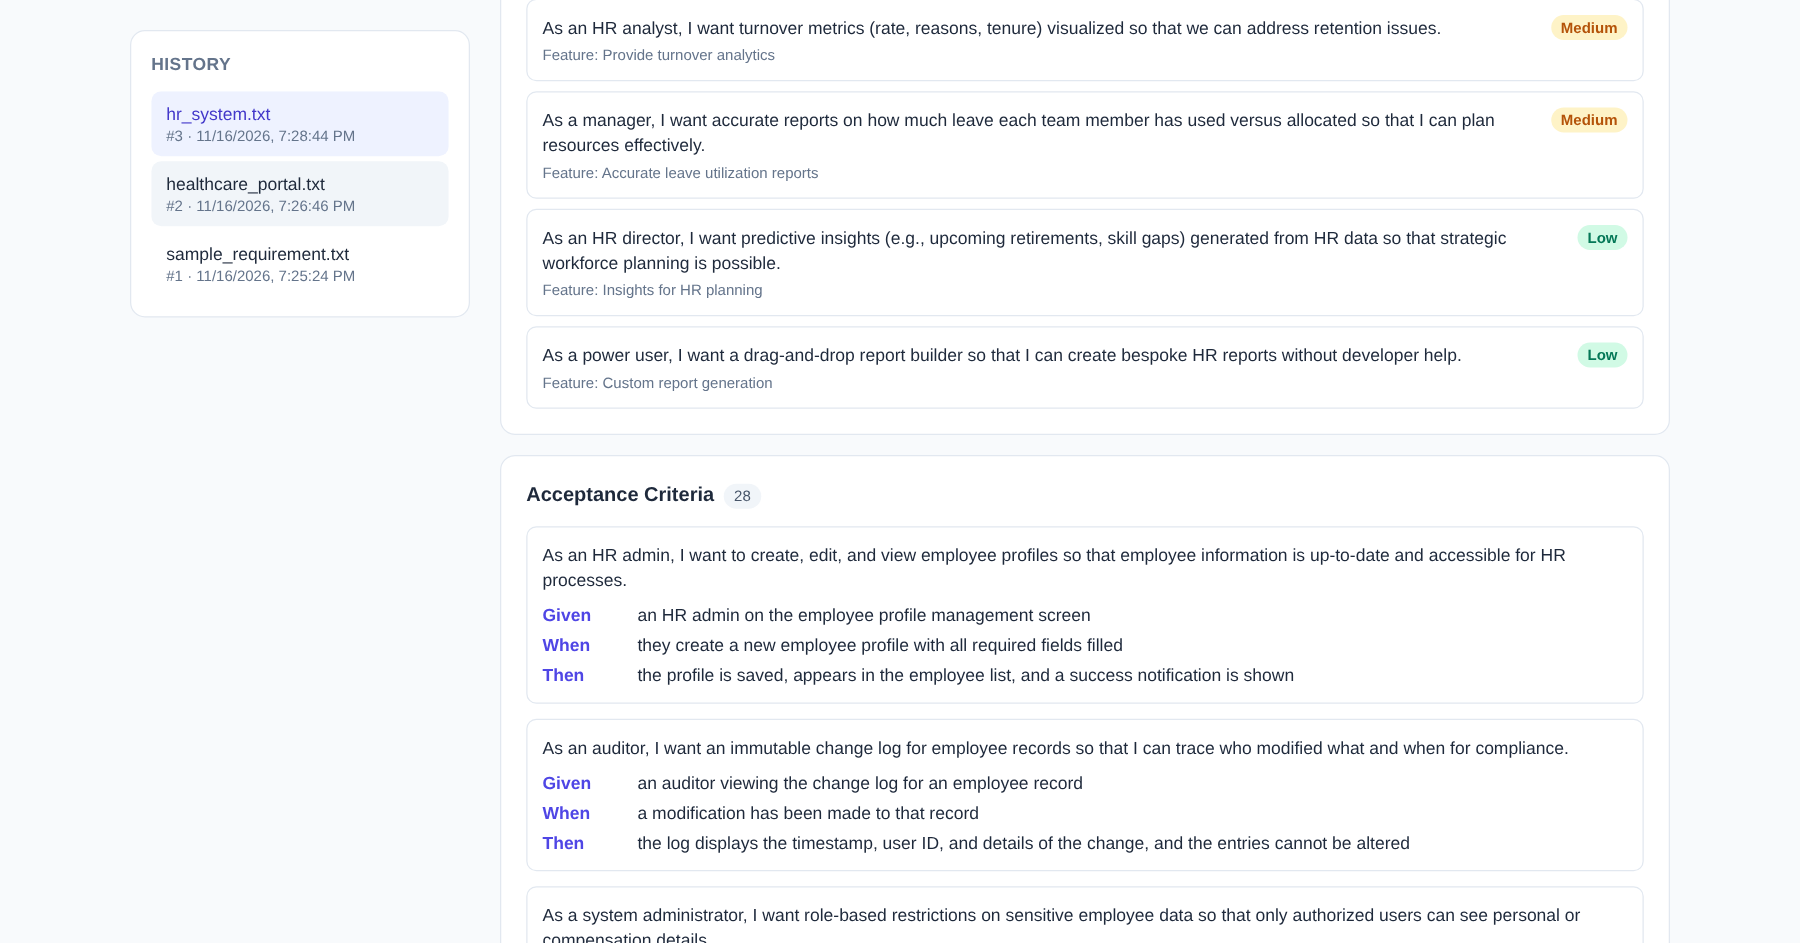
\includegraphics[width=433pt]{assets/report_output.png}
\caption{Final structured report rendered in the frontend, showing requirements, user stories, acceptance criteria and flagged risks.}
\label{fig:reportview}
\end{figure}

\begin{table}[H]
\centering
\caption{Summary of Test-Run Results}
\label{tab:results}
\begin{tabularx}{\textwidth}{|p{5.6cm}|X|}
\hline
\textbf{Evaluation Metric} & \textbf{Observed Value (e-commerce / healthcare / HR)} \\
\hline
Functional requirements extracted & \mFR\ requirements \\
\hline
Non-functional requirements extracted & \mNFR\ requirements \\
\hline
User stories generated & \mUS\ stories \\
\hline
Acceptance criteria generated & \mAC\ criteria sets \\
\hline
Ambiguities flagged & \mAMB\ ambiguities \\
\hline
Risks flagged & \mRISK\ risks \\
\hline
End-to-end processing time & \mTIME\ seconds \\
\hline
\end{tabularx}
\end{table}

The values in Table 5.1 were measured from one controlled run of the final
pipeline on each of the three sample documents through the
\texttt{/analyze} endpoint, using \texttt{openai/gpt-oss-120b} on Groq
because \texttt{llama-3.3-70b-versatile} was no longer available.

\setcounter{section}{2}
\section{Technical Findings from Execution Evidence}
The FastAPI screenshots confirm successful HTTP 200 responses for full
analysis and run-history retrieval. The response structure contains a
run\_id and a nested report, which proves that report assembly and SQLite
persistence execute in the same workflow. The frontend confirms that the
backend/frontend contract is aligned, and the earlier formatting defect in
acceptance criteria was fixed (Section 4.5). The upload API now stores
files under server-generated names with an extension allow-list, a 5~MB
size limit and path confinement. The full pipeline is still synchronous, so
it should be moved to a background queue for concurrent use. The backend
is covered by \mPY\ \texttt{pytest} tests and the frontend by \mJS\
\texttt{vitest} tests, all passing.

\section{Observations}
Across the three sample documents, the Requirement Analysis and
Classification agents consistently separated functional from non-functional
requirements correctly. The Risk \& Ambiguity agent flagged the
intentionally vague phrasing in the samples (for example, unqualified
words like ``fast'' or ``secure'') and proposed specific, measurable
replacements; precision and recall were not measured, and the 0.40
threshold was chosen empirically on these three documents. The main source
of variation was in how granular the generated user stories were for very
broad requirements, which was addressed by refining the prompt to ask for
one story per distinct feature rather than per sentence.

\section{Project Repository}
The complete source code is available on GitHub, as shown in Figure 5.3.

\begin{figure}[H]
\centering
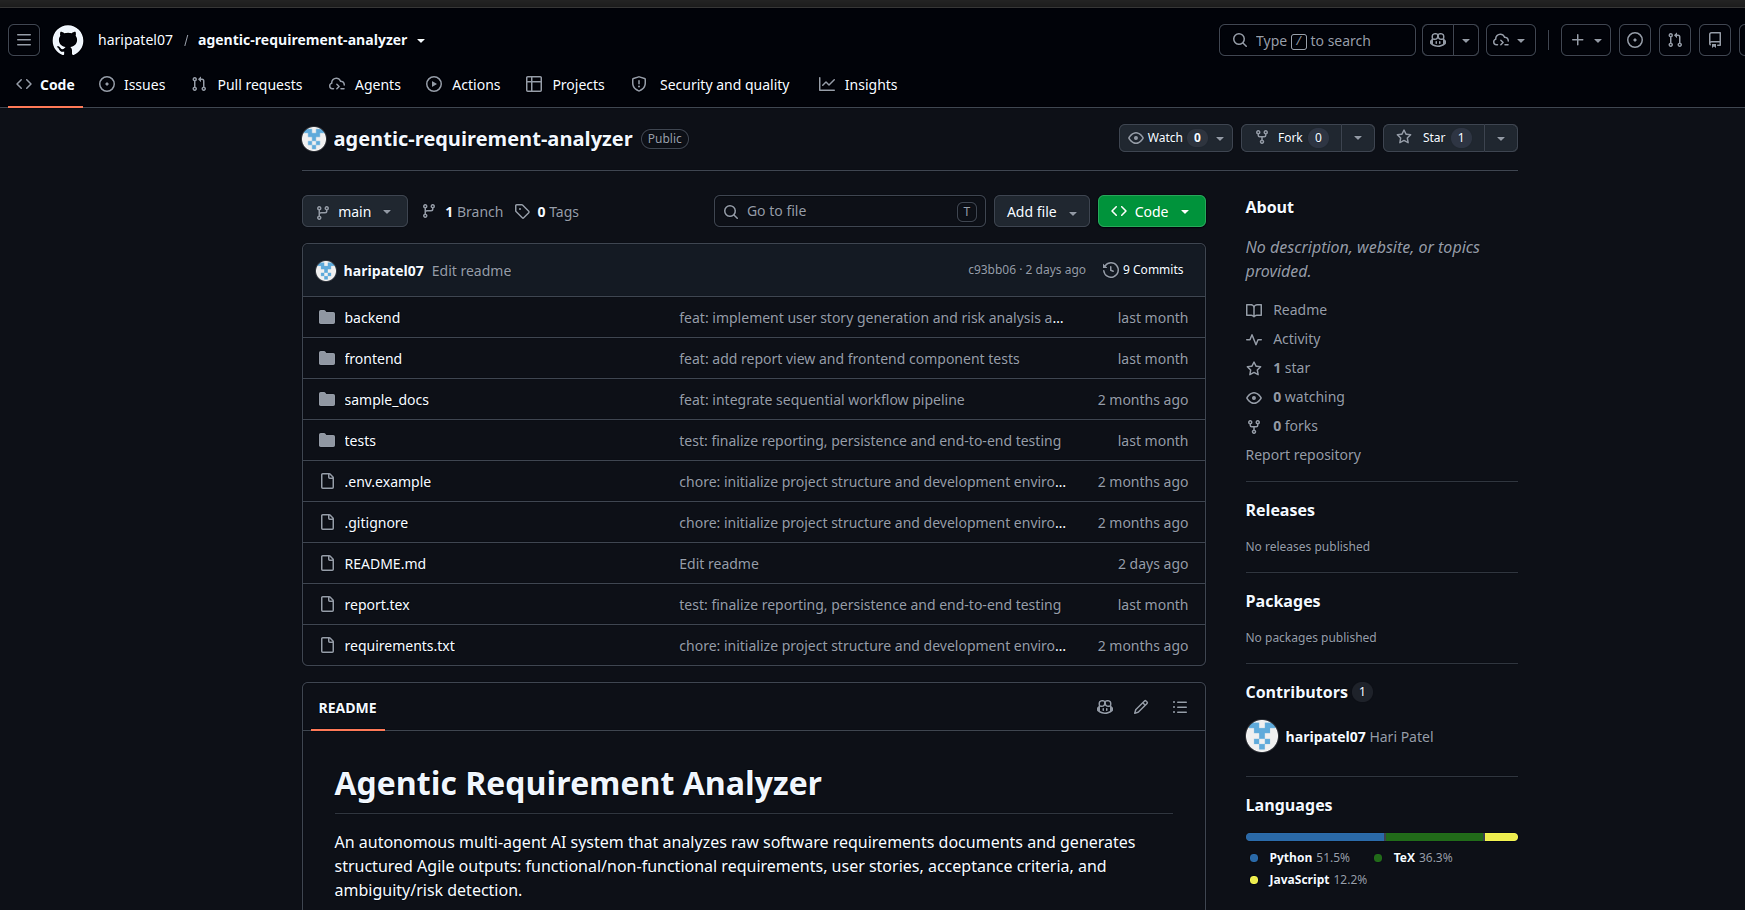
\includegraphics[width=0.9\textwidth]{assets/github_repo.png}
\caption{Agentic Requirement Analyzer repository on GitHub.}
\label{fig:githubrepo}
\end{figure}
\end{document}
